
%(BEGIN_QUESTION)
% Copyright 2010, Tony R. Kuphaldt, released under the Creative Commons Attribution License (v 1.0)
% This means you may do almost anything with this work of mine, so long as you give me proper credit

Examine this P\&ID for a temperature control system in a vessel heated by steam.  The steam control valve is air-to-close (fail-open):

$$\includegraphics[width=15.5cm]{i03786x01.eps}$$

Determine the effect on the control system's regulation of temperature inside the vessel if the incoming feed temperature cools down to a lower value.  Assume all loop components are properly configured, that the controller is well-tuned, and that a significant amount of time has passed since the temperature drop.  Compare these conditions with what they were before the process change:

\begin{itemize}
\item{} Steam valve will: {\it open up} further, {\it close down} more, or {\it remain in the same position} 
\vskip 10pt
\item{} I/P output pressure signal will: {\it increase}, {\it decrease}, or {\it remain the same} 
\end{itemize}

\underbar{file i03786}
%(END_QUESTION)





%(BEGIN_ANSWER)

\begin{itemize}
\item{} Steam valve will: {\bf open up further}
\vskip 5pt
\item{} I/P output pressure signal will: {\bf decrease}
\end{itemize}

%(END_ANSWER)





%(BEGIN_NOTES)

{\bf This question is intended for exams only and not worksheets!}.

%(END_NOTES)


